\begin{thm}{061}{\hosi 7}{関西医科大 後期 (2019)}
 実数$a,b$を用いて表される4次方程式 $x^4+4ax^3+2(2b-1)x^2+4ax+1=0$ の全ての解が、複素数平面上で原点から等距離にある。この条件を満たす解が存在するような$a,b$の条件を求め、点(a,b)の存在範囲を$ab$平面上に図示せよ。
\end{thm}

与えられた4次方程式は明らかに$x=0$を解に持たないから$x^2$で割って、
\begin{align*}
 x^4+4ax^3+2(2b-1)x^2+4ax+1&=0 \quad\cdots(\text{*}) \\
 \dou\quad x^2+\frac{1}{x^2}+4a\left(x+\frac{1}{x}\right)+4b-2&=0 \quad\cdots\text{\marunum{1}}
\end{align*}
よって$x=z$が解ならば$x=\dfrac{1}{z}$も解になることが明らかであり、条件より$|z|=\dfrac{1}{|z|}$だから$|z|=1$が従う。したがって、(*)の4解が原点から等距離であることは、(*)の4解の絶対値が1であることと同値である。さて\marunum{1}にて$t=x+\dfrac{1}{x}$とおくと$t^2=x^2+2+\dfrac{1}{x^2}$から、
\[ \marunum{1} \,\dou\, t^2+4at+4(b-1)=0 \quad\cdots\marunum{2} \]
さらに$x=\cos\theta+i\sin\theta$とおくと$t=2\cos\theta$なので、$-2\le t\le 2$の範囲の実数となる、よって、\marunum{2}の全ての実数解は区間$[-2,2]$上になければならない。このような$(a,b)$の条件を考える。$f(t)=t^2+4at+4(b-1)$とする。

$\marunum{2}$の判別式$D$について
\[ D=16a^2-16(b-1)\ge 0 \quad\dou\quad a^2+1\ge b \]

放物線$f(t)=(t+2a)^2+4(b-1)-4a^2$の軸が区間$[-2,2]$上にあることが必要で、
\[ -2\le -2a \le 2 \quad\dou\quad -1\le a\le 1 \]

端点について$f(-2)\ge 0$かつ$f(2)\ge 0$から、
\[ 2a+b\ge 0 \,\text{かつ}\, -2a+b\ge 0 \quad\dou\quad b\ge\max{2a,-2a} \]

よって$(a,b)$の存在範囲の必要条件として次を得る。ただし境界は全て含む。
\begin{figure}[H]
 \centering
 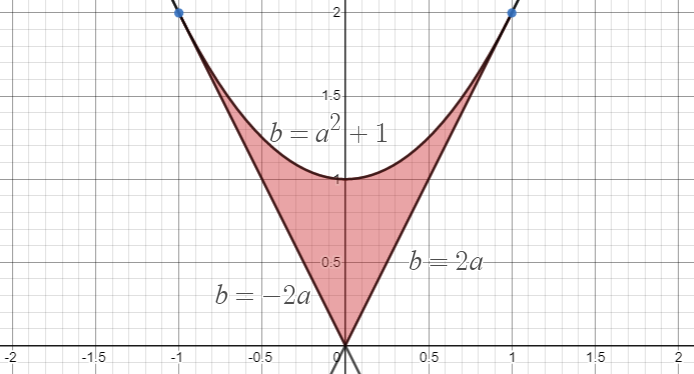
\includegraphics[width=0.8\linewidth]{../problems/Q_061/A_061.png}
\end{figure}

逆にこの領域上の点$(a,b)$は全て条件を満たす。$\marunum{2}$が区間$[-2,2]$上の実数解を持つので、その解を$p,q\,(\in\,[-2,2])$としよう\footnote{編集者註: $p=q$の場合も含む。}。このとき、
\[ \frac{p}{2}=\cos\theta_p \,,\,\, \frac{q}{2}=\cos\theta_q \]
なる$\theta_p, \theta_q\,\in[0,\pi]$がただ一つ存在する。すると(*)の4解は、
\[ z_p=\cos\theta_p+i\sin\theta_p \,,\,\, z_q=\cos\theta_q+i\sin\theta_q \]
として$x=z_p, \overline{z_p}, z_q, \overline{z_q}$ですべて与えられ、実際に原点から等距離にある。よって求める領域は先の領域である。